\documentclass[../thesis.tex]{subfiles}

\begin{document}
\vspace{-1\baselineskip}

\section{The Standard Model}
\label{sec:SM}
The Standard Model of Physics (\acs{SM}) \citep{theory:SM} is currently the most successful formalism to describe the physical world at a microscopic scale by providing descriptions for all currently known elementary particles, along with three out of four fundamental forces (electromagnetism, weak force, strong force) with the exception of gravity. The \acs{SM} is however not perfect, and there remains unanswered questions that require development and discovery of new physics beyond the Standard Model (\acs{BSM}). This chapter describes an overview of important components within the \acs{SM} and relevant \acs{BSM} aspects for this analysis.

%- limitations: gravity \& general relativity, arbitrary free parameters
\subsection{Elementary particles}
Elementary particles in the \acs{SM} can be classified into two groups: bosons consisting of particles following Bose-Einstein statistics with integer spin, and fermions consisting of particles following Fermi-Dirac statistics with half-integer spin. Fermions are the building blocks of composite particles and consequently all known matter, and can be further classified into quarks \& leptons. Bosons act as force mediators for all fundamental forces described by the \acs{SM}, and can either be a scalar boson with spin $0$ or vector gauge bosons with spin $1$. For each elementary particle, there also exists a corresponding antiparticle with identical mass and opposite charge (electric or color). \autoref{fig:smparticles} shows all known elementary particles in the \acs{SM}.

\begin{figure}[!htb]
\begin{center}
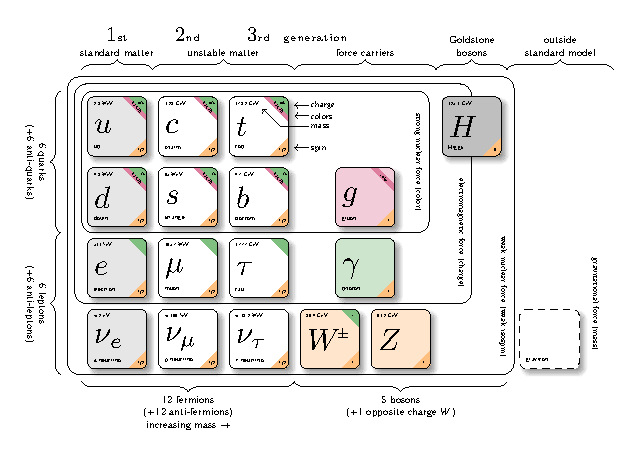
\includegraphics[width=\linewidth]{fig/theory_smparticles.pdf}
\caption[Particles within the SM and their properties.]{\label{fig:smparticles}Particles within the \acs{SM} and their properties \citep{theory:smparticles}.}
\end{center}
\end{figure}

\subsubsection*{Fermions}
Fermions consist of quarks and leptons with six flavors each, grouped into three generations of doublets. The six quark flavors are up ($u$), down ($d$), charm ($c$), strange ($s$), bottom ($b$) and top ($t$), arranged in increasing order of mass. The quark flavors form three doublets $(u,d)$, $(c,s)$ and $(t,b)$, with each doublet containing one quark with electric charge of $+2/3$ ($u$, $s$, $t$), and the other with charge of $-1/3$ ($d$, $c$, $b$). Each quark also possesses a property known as color charge, with possible values of red ($R$), green ($G$), blue ($B$) or their corresponding anticolor ($\bar{R}$, $\bar{G}$, $\bar{B}$). Color charge follows color confinement rules, which allows only configurations of quarks with total neutral color charge to exist in isolation. Neutral charge configurations can be formed from either a set of three colors $(R,G,B)$, a set of a color and its anticolor $(q,\bar{q})$, or any combination of the two. Consequently, quarks can only exist in bound states called hadrons and no isolated quark can be found in a vacuum. Quarks are the only elementary particles in the \acs{SM} that can interact with all four fundamental forces.

The three leptons doublets consist of three charged leptons: electron ($e$), muon ($\mu$), tau ($\tau$), and their respective neutrino flavors: electron neutrino ($\nu_e$), muon neutrino ($\nu_\mu$), tau neutrino ($\nu_\tau$). Charged leptons carry an electric charge of $-1$, while their antiparticles carry the opposite charge ($+1$) and their corresponding neutrino flavors carry no charge. Charged leptons interact with all fundamental forces except the strong force, while neutrinos only interact with the weak force and gravity.

\subsubsection*{Bosons}
The \acs{SM} classifies bosons into two types: one scalar boson with spin $0$ known as the Higgs ($H$) boson, and vector gauge bosons with spin $1$ known as gluons ($g$), photon ($\gamma$), $W^\pm$ and $Z$ bosons. Gluons and photon are massless, while the $W^\pm$, $Z$ and $H$ bosons are massive. Each vector gauge boson serves as the mediator for a fundamental force described by the \acs{SM}. Gluons are massless particles mediating the strong interaction by carrying color charges between quarks following quantum chromodynamics (\acs{QCD}). Each gluon carries a non-neutral color charge out of eight linearly independent color states in the gluon color octet \citep{theory:gellmann}. Photon is the massless and charge-neutral mediator particle for the electromagnetic interaction following quantum electrodynamics (\acs{QED}). The $W^\pm$ and $Z$ bosons are massive mediator particles for the weak interaction, with the $W^\pm$ boson carrying an electric charge of $\pm 1$ while the $Z$ boson is charge neutral.

Other than the vector gauge boson, the only scalar boson in the \acs{SM} is the massive and charge neutral Higgs boson. The Higgs boson does not mediate any fundamental force like vector bosons, but serve to provide the rest mass for all massive elementary particles in the SM through the Higgs mechanism described in section \ref{sec:higgs}.

\subsubsection*{Top quark}
\label{sec:top}

As of now, the top quark ($t$) is the heaviest particle in the \acs{SM} with mass of about 173 GeV \citep{PDG}. For comparison, the heaviest boson, the Higgs boson, possesses mass of 125 GeV and the second most massive fermion, the $b$-quark has mass of about 4.2 GeV. This gives the top quark the strongest Yukawa coupling to the Higgs boson ($y_t \approx 1$) \citep{theory:top_coupling} and exotic resonances in many proposed \acs{BSM} models \citep{theory:top_exotics,theory:top_exotics2,theory:top_exotics3,theory:top_exotics4}, making the top quark and its processes attractive vehicles with which to probe new physics.

\begin{wrapfigure}{r}{0.5\textwidth}
%\begin{figure}[!htb]
\begin{center}
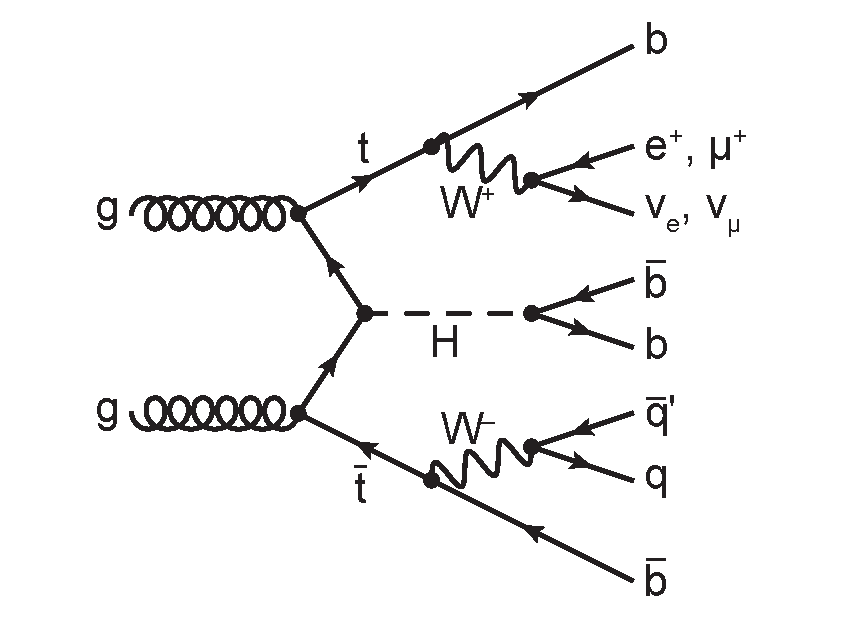
\includegraphics[width=\linewidth]{fig/theory_tt_decay.pdf}
\caption[Feynman diagram for \ttbar production and subsequent decay processes. Top quark decays into a $W$-boson and $b$-quark, and $W$-boson can decay to a $q\bar{q}$ or a $\ell\nu_\ell$ pair.]{\label{fig:theory:tt_decay}Feynman diagram for \ttbar production and subsequent decay processes \citep{theory:ttH_Hbb}. Top quark decays into a $W$-boson and $b$-quark, and $W$-boson can decay to a $q\bar{q}$ or a $\ell\nu_\ell$ pair.}
\end{center}
%\end{figure}
\end{wrapfigure}

Due to its mass, the top quark has a very short lifetime of $10^{-24}$ s \citep{PDG} and decays before it can hadronize following color confinement. The top quark decays to a $W$ boson and a $b$-quark with a branching ratio of almost $100\%$. The $W$ boson can subsequently decay hadronically or leptonically (\autoref{fig:theory:tt_decay}), with branching ratios of approximately $68\%$ and $32\%$ respectively. All lepton flavors have similar branching ratios during a leptonic $W$ decay, assuming lepton universality.

\textcolor{red}{additional section on 4top production?}


\subsection{Mathematical formalism}
The \acs{SM} can be described within the formalism of quantum field theory (\acs{QFT}) with the Lagrangian
\begin{equation}
\mathcal{L}_\mathrm{SM} = \mathcal{L}_\mathrm{QCD} + {\underbrace{(\mathcal{L}_\mathrm{gauge}+\mathcal{L}_\mathrm{fermion}+\mathcal{L}_\mathrm{Higgs}+\mathcal{L}_\mathrm{Yukawa})}_{\mathcal{L}_\mathrm{EW}}}
\end{equation}
where $\mathcal{L}_\mathrm{QCD}$ is the \acs{QCD} term and $\mathcal{L}_\mathrm{EW}$ is the electroweak (\acs{EW}) term of the Lagrangian. Formalism of \acs{QFT} within the \acs{SM} treats particles as excitations \citep{theory:qft} of their corresponding quantum fields i.e. fermion field $\psi$, electroweak boson fields $W_{1,2,3}$ \& $B$, gluon fields $G_\alpha$ and Higgs field $\phi$.

The foundation of modern \acs{QFT} involves gauge theory. A quantum field has gauge symmetry if there exists a continuous gauge transformation that when applied to every point in a field (local gauge transformation) leaves the field Lagrangian unchanged. The set of gauge transformations of a gauge symmetry is the symmetry group of the field which comes with a set of generators, each with a correspoding gauge field. Under \acs{QFT}, the quanta of these gauge fields are called gauge bosons.

The \acs{SM} Lagrangian is gauge invariant under global Poincar\'e symmetry and local $SU(3)_C \times SU(2)_L \times U(1)_Y$ gauge symmetry, with the $SU(3)_C$ symmetry group corresponding to the strong interaction and $SU(2)_L \times U(1)_Y$ to the \acs{EW} interaction. Global Poincar\'e symmetry ensures that $\mathcal{L}_\mathrm{SM}$ satisfies translational symmetry, rotational symmetry and Lorentz boost frame invariance \citep{theory:symmetry}. These symmetries give rise to corresponding conservation laws, which lead to conservation of momentum, angular momentum and energy in the \acs{SM} as a result of Noether's theorem.

\subsubsection{Quantum chromodynamics}
Quantum chromodynamics is a non-Abelian gauge theory i.e. Yang-Mills theory \citep{theory:yangmills,theory:yangmills2} describing the strong interaction between quarks in the \acs{SM} with the gauge group $SU(3)_C$, where $C$ represents conservation of color charge under $SU(3)_C$ symmetry. According to \acs{QFT}, quarks can be treated as excitations of the corresponding quark fields $\psi$.
%Quark fields are invariant under $SU(3)_C$ transformation
%\begin{equation}
%\psi \rightarrow e^{i\theta(x)T_a} \psi
%\end{equation}
%where .
The free Dirac Lagrangian for the quark fields
\begin{equation}
\mathcal{L}_0=\bar{\psi}(i\gamma^\mu\partial_\mu-m)\psi
\end{equation}
is invariant under global $SU(3)$ symmetry, but not under local $SU(3)_C$ symmetry.
To establish invariance under local $SU(3)_C$ symmetry, the gauge covariant derivative $D_\mu$ is defined so that
\begin{equation}
D_\mu \psi = (\partial_\mu-ig_sG^a_\mu T_a)\psi,
\end{equation}
where $g_s=\sqrt{4\pi\alpha_s}$ is the \acs{QCD} coupling constant, $G^a_\mu(x)$ are the eight gluon fields, and $T_a$ are generators of $SU(3)_C$, represented as $T_a=\lambda_a/2$ with $\lambda_a$ being the eight Gell-Mann matrices \citep{theory:gellmann}.
%that transform under $SU(3)_C$ as
%\begin{equation}
%G_\mu^a \rightarrow e^{iT_a\theta_a(x)}\left( G_\mu^a+\frac{i}{g_s}\partial_\mu \right)e^{-iT_a\theta_a(x)}
%=G_\mu^a - \frac{1}{g_s}\partial_\mu\theta_a(x)-f_{abc}\theta_b(x)G_\mu^c.
%\end{equation} 
Let the gluon field strength tensors $G^a_{\mu \nu}$ be
\begin{equation}
G_{\mu \nu}^a \equiv \partial_\mu G^a_\nu - \partial_\nu G^a_\mu - g_s f^{abc} G^b_\mu G^c_\nu,
\end{equation}
where $f^{abc}$ are the structure constants of $SU(3)_C$. The gauge invariant \acs{QCD} Lagrangian can then be written as
\begin{equation}
\begin{aligned}
\mathcal{L}_\text{QCD}
&=\bar{\psi}(i\gamma^\mu D_\mu-m)\psi - \frac{1}{4} G_{\mu \nu}^a G_a^{\mu \nu} \\
&= 
\underbrace{
-\frac{1}{4} G_{\mu \nu}^a G_a^{\mu \nu}
}_{\substack{\text{gluon kinematics}\\ \text{\& self-interaction}}}
+\underbrace{\vphantom{\frac{1}{4}}
\bar{\psi}\left( i\gamma^\mu \partial\mu-m \right)\psi
}_{\substack{\text{quark kinematics}\\ \text{\& masses}}}
+\underbrace{\vphantom{\frac{1}{4}}
\bar{\psi}^i\left( g_s \gamma^\mu (T_a)_{ij} G^a_\mu \right)\bar{\psi}^j
}_\text{quark-gluon interaction},
\end{aligned}
\end{equation}
where $i$, $j$ are color indices with integer values from $1$ to $3$. Gluons are forced to be massless from the lack of a gluon mass term to maintain gauge invariance for the Lagrangian.

\subsubsection{Electroweak theory}
The electroweak interaction is the unified description of the weak interaction and electromagnetism under the $SU(2)_L \times U(1)_Y$ symmetry group, where $L$ represents the left-handed chirality of the weak interaction and $Y$ represents the weak hypercharge quantum number.
%The quantum number associated with the weak chirality is the weak isospin $I$. The \acs{EW} quantum numbers are connected by the Gell-Mann-Nishijima relation
%\begin{equation}
%Q = I_3 + Y/2
%\end{equation}
%where $Q$ is the electric charge and $I_3$ is the third component of weak isospin $I$.
Fermions can have either left-handed or right-handed chirality with the exception of neutrinos which can only have left-handed chirality in the \acs{SM}, and can be divided into left-handed doublets and right-handed singlets
\begin{equation}
\begin{aligned}
\psi_L &= \displaystyle\binom{\nu_e}{e_L}, \displaystyle\binom{\nu_\mu}{\mu_L}, \displaystyle\binom{\nu_\tau}{\tau_L}, \displaystyle\binom{u_L}{d_L}, \displaystyle\binom{c_L}{s_L}, \displaystyle\binom{t_L}{b_L} \\
\psi_R &= e_R\text{, }\mu_R\text{, }\tau_R\text{, }u_R\text{, }d_R\text{, }c_R\text{, }s_R\text{, }t_R\text{, }b_R.
\end{aligned}
\end{equation}
%Both left-handed and right-handed fermion fields are invariant under $U(1)_Y$ transformation
%\begin{equation}
%\psi \rightarrow e^{iY\theta(x)/2} \psi.
%\end{equation}
Similar to \acs{QCD}, to establish invariance under local $U(1)_Y$ symmetry, the $U(1)_Y$ gauge covariant derivative $D_\mu$ is defined as
\begin{equation}
D_\mu \phi = \left( \partial_\mu -ig' \frac{Y}{2} B_\mu \right) \psi
\end{equation}
where $g'$ is the $B_\mu$ coupling constant and $B_\mu(x)$ is a vector gauge field that transforms under $U(1)_Y$ as
\begin{equation}
B_\mu \rightarrow B_\mu + \frac{1}{g'}\partial_\mu \theta(x).
\end{equation}
%The Lagrangian
%\begin{equation}
%\mathcal{L} = \bar{\psi}(i\gamma^\mu D_\mu-m)\psi 
%= \bar{\psi}\left( i\gamma^\mu\partial_\mu-m \right)\psi + \bar{\psi}\left( g\frac{Y}{2}B_\mu \right)\psi
%\end{equation}
%is then invariant under local $U(1)_Y$ symmetry.\\
Right-handed fermion singlets are not affected by $SU(2)_L$ transformation, so the fermion fields $\psi$ transform under $SU(2)_L$ as
\begin{equation}
\begin{aligned}
\psi_L &\rightarrow e^{iI_3 \vec{\theta}(x)\cdot\vec{\sigma}/2} \psi_L \\
\psi_R &\rightarrow \psi_R.
\end{aligned}
\end{equation}
where $\vec{\sigma}/2$ are generators of $SU(2)_L$ with $\vec{\sigma}$ being the Pauli matrices. In order to preserve local symmetry, let the gauge covariant derivative for $SU(2)_L$ be
\begin{equation}
D_\mu \psi_L = \left( \partial_\mu - ig\frac{\sigma_i}{2}W_\mu^i \right) \psi_L
\end{equation}
where $W_\mu^i (x)$ ($i=1,2,3$) are three boson gauge fields that transform under $SU(2)_L$ as
\begin{equation}
W_\mu^i \rightarrow e^{i\displaystyle\frac{\sigma_i}{2}\theta_i(x)} \left( W_\mu^i+\frac{i}{g}\partial_\mu \right) e^{-i\displaystyle\frac{\sigma_i}{2}\theta_i(x)}
= W_\mu^i + \frac{2}{g}\partial_\mu \theta_a(x) + \epsilon^{ijk}\theta_j(x) W_\mu^k,
\end{equation}
with $g$ as the $W^i_\mu$ gauge coupling constant, and $\epsilon^{ijk}$ as the $SU(2)_L$ structure constant. The gauge covariant derivative for $SU(2)_L \times U(1)_Y$ can then be written as
\begin{equation}
\begin{aligned}
\label{eq:EW_cov}
D_\mu \psi_L &= \left( \partial_\mu - ig'\frac{Y_L}{2}B_\mu - ig\frac{\sigma_i}{2}W_\mu^i \right) \psi_L \\
D_\mu \psi_R &= \left( \partial_\mu - ig'\frac{Y_R}{2}B_\mu \right) \psi_R.
\end{aligned}
\end{equation}

Similar to \acs{QCD}, the kinetic term is added by defining field strengths for the four gauge fields
\begin{equation}
\begin{aligned}
B_{\mu \nu}   &\equiv \partial_\mu B_\nu - \partial_\nu B_\mu \\
W_{\mu \nu}^i &\equiv \partial_\mu W^i_\nu - \partial_\nu W^i_\mu - g e^{ijk} W^j_\mu W^k_\nu.
\end{aligned}
\end{equation}
The local $SU(2)_L \times U(1)_Y$ invariant \acs{EW} Lagrangian is then \citep{theory:ew}
\begin{equation}
\begin{aligned}
\mathcal{L}_\text{EW} &= i\bar{\psi}(\gamma^\mu D_\mu)\psi - \frac{1}{4}W^i_{\mu\nu}W_i^{\mu\nu} - \frac{1}{4}B_{\mu\nu}B^{\mu\nu} \\
&= \underbrace{\vphantom{\left(\frac{Y}{2}\right)}
i\bar{\psi}\left(\gamma^\mu\partial_\mu\right)\psi
}_{\substack{\text{fermion}\vphantom{\frac{1}{4}}\\ \text{kinematics}}}
\underbrace{
-\bar{\psi}\left(\gamma^\mu g'\frac{Y}{2}B_\mu\right)\psi - \bar{\psi}_L\left(\gamma^\mu g\frac{\sigma_i}{2}W_\mu^i\right)\psi_L
}_\text{fermion-gauge boson interaction}
\underbrace{\vphantom{\left(\frac{Y}{2}\right)}
-\frac{1}{4}W^i_{\mu\nu}W_i^{\mu\nu} - \frac{1}{4}B_{\mu\nu}B^{\mu\nu}
}_{\substack{\text{boson kinematics}\vphantom{\frac{1}{4}}\\ \text{\& self-interaction}}}.
\end{aligned}
\end{equation}
Under $\approx 159.5$ GeV, the \acs{EW} symmetry $SU(2)_L\times U(1)_Y$ undergoes spontaneous symmetry breaking \citep{theory:ew_scale} into $U(1)_\text{QED}$ symmetry, which corresponds to a separation of the weak and electrodynamic forces. Electroweak spontaneous symmetry breaking replaces the four massless and similarly-behaved \acs{EW} gauge bosons $B_\mu$ and $W_\mu^i$ with the \acs{EM} boson $\gamma$ and the weak bosons $Z/W^\pm$, as well as giving the $Z$ and $W^\pm$ bosons masses via the Higgs mechanism. This is due to a specific choice of gauge for the Higgs field leading to the reparameterization of the \acs{EW} bosons $B_\mu$ and $W_\mu^i$ to $W^\pm$/$Z$/$\gamma$ using the relations
\begin{equation}
\begin{aligned}
\label{eq:EW_repara}
W^\pm_\mu &\equiv \frac{1}{\sqrt{2}}\left(W^1_\mu \mp iW^2_\mu\right) \\ 
\begin{pmatrix}
A_\mu \\ Z_\mu
\end{pmatrix}
&\equiv \begin{pmatrix}
\cos \theta_\text{W} & \sin \theta_\text{W} \\
-\sin \theta_\text{W} & \cos \theta_\text{W}
\end{pmatrix}
\begin{pmatrix}
B_\mu \\ W_\mu^3
\end{pmatrix}
\end{aligned}
\end{equation}
where $\theta_\text{W}\equiv\cos^{-1}\left(g/\sqrt{g^2+g'^2}\right)$ is the weak mixing angle. The boson kinetic term can also be refactorized to extract cubic (three vertices) and quartic (four vertices) self-interactions among the gauge bosons \citep{theory:ew}. The Lagrangian can then be rewritten as
\begin{equation}
\begin{aligned}
\label{eq:EW_L}
\mathcal{L} &=
\underbrace{\vphantom{\displaystyle\frac{e}{2\sin\theta_\text{W}}}
eA_\mu\bar{\psi}\left(\gamma^\mu Q\right)\psi
}_\text{electromagnetism}
+\underbrace{
\displaystyle\frac{e}{2\sin\theta_\text{W}\cos\theta_\text{W}}\bar{\psi}\gamma^\mu\left(v_f-a_f\gamma_5 \right)\psi Z_\mu
}_\text{neutral current interaction} \\
&+\underbrace{
\displaystyle\frac{g}{2\sqrt{2}}\mathlarger{\sum}_{\psi_L}
\left[ \bar{f}_2\gamma^\mu\left(1-\gamma_5\right)f_1 W_\mu^+ + \bar{f}_1\gamma^\mu\left(1-\gamma_5\right)f_2 W_\mu^- \right]
}_\text{charged current interaction} \\
&+\mathcal{L}_\text{kinetic}+\underbrace{\vphantom{\frac{1}{4}}
\mathcal{L}_\text{cubic}+\mathcal{L}_\text{quartic}
}_\text{boson self-interaction}
\end{aligned}
\end{equation}
where $\gamma_5=i\gamma^0\gamma^1\gamma^2\gamma^3$ is the chirality projection operator, $a_f=I_3$, $v_f=I_3(1-4|Q|\sin^2\theta_\text{W})$ and $f_1$, $f_2$ are up and down type fermions of a left-handed doublet.

\subsubsection{Higgs mechanism}
\label{sec:higgs}
So far, the \acs{EW} bosons are massless since the mass terms $-m\bar{\psi}\psi$ for fermions and $-mA^\mu A_\mu$ for bosons are not invariant under the \acs{EW} Lagrangian symmetries. The particles must then acquire mass under another mechanism. The Brout-Engler-Higgs mechanism \citep{theory:higgs1,theory:higgs2,theory:brout_englert} was introduced in 1964 to rectify this issue and verified in 2012 with the discovery of the Higgs boson \citep{theory:higgs_atlas,theory:higgs_cms}.

The Higgs potential is expressed as
\begin{equation}
V(\phi^\dagger\phi) = \mu^2\phi^\dagger\phi+\lambda(\phi^\dagger\phi)^2
\end{equation}
where $\mu^2$ and $\lambda>0$ are arbitrary parameters, and the $SU(2)_L$ doublet $\phi=\binom{\phi^+}{\phi^0}$ is the Higgs field with complex scalar fields $\phi^+$ and $\phi^0$ carrying $+1$ and $0$ electric charge respectively. The Lagrangian for the scalar Higgs field is
\begin{equation}
\mathcal{L}_H = \left(\partial_\mu \phi\right)^\dagger \left(\partial^\mu \phi\right) - V\left(\phi^\dagger\phi\right).
\end{equation}
%which is invariant under local $U(1)$ transformation
%\begin{equation}
%\phi \rightarrow e^{i\theta(x)}\phi.
%\end{equation}
Since the potential $V(\phi^\dagger\phi)$ is constrained by $\lambda>0$, the ground state is solely controlled by $\mu$. If $\mu^2>0$, the ground state energy is $\phi=0$, and the \acs{EW} bosons would remain massless. If $\mu^2<0$, the ground state is
\begin{equation}
|\phi|^2 = -\displaystyle\frac{\mu^2}{2\lambda} \equiv \displaystyle\frac{v^2}{\sqrt{2}},
\end{equation}
where $v$ is defined as the vacuum expectation value (\acs{VEV}). The standard ground state for the Higgs potential without loss of generality can be chosen as $\phi(0) = 1/\sqrt{2}\binom{0}{v}$.
%ball at the top of the hat = rotational symmetry
%ball falls down and settles on a point of lowest energy = break symmetry
%\textcolor{red}{sombrero potential pic}\\

\begin{figure}[!htb]
\begin{center}
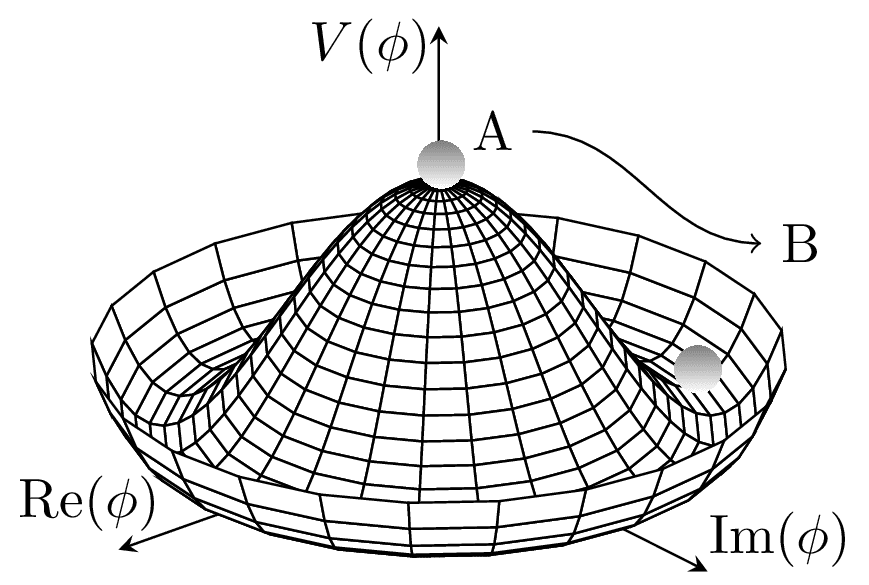
\includegraphics[width=0.5\linewidth]{fig/theory_higgs_potential.png}
\caption[Illustration of a common representation of the Higgs potential. Before SSB, the ground state $\phi(0)$ is located at A which is symmetric with respect to the potential. A perturbation to this state fixes the ground state energy $|\phi(0)|^2$ to a particular value at B, "spontaneously" breaking the symmetry and degeneracy in $|\phi(0)|^2$.]{\label{fig:theory:higgs_pot}Illustration of a common representation of the Higgs potential \citep{theory:higgs_pot}. Before \acs{SSB}, the ground state $\phi(0)$ is located at A which is symmetric with respect to the potential. A perturbation to this state fixes the ground state energy $|\phi(0)|^2$ to a particular value at B, "spontaneously" breaking the symmetry and degeneracy in $|\phi(0)|^2$.}
\end{center}
\end{figure}

Having $U(1)$ symmetry allows any $-e^{i\theta}\sqrt{\mu^2/\lambda}$ to be a ground state energy for the Higgs Lagrangian. This degeneracy results in spontaneous symmetry breaking of the $SU(2)_L\times U(1)_Y$ symmetry into $U(1)_\text{\acs{EM}}$ symmetry when the Higgs field settles on a specific vacuum state as a result of a perturbation or excitation (\autoref{fig:theory:higgs_pot}). The spontaneous symmetry breaking introduces three massless (Nambu-Goldstone \citep{theory:nambu_goldstone}) vector gauge boson $\xi$ and a massive scalar boson $\eta$, each corresponds to a generator of the gauge group. The vector field for $\xi$ and $\eta$ are real fields parameterized as $\xi \equiv \phi^+\sqrt{2}$ and $\eta \equiv \phi^0\sqrt{2}-v$ \citep{theory:higgs_physics}. The Higgs field now becomes
\begin{equation}
\phi=\frac{v+\eta+i\xi}{\sqrt{2}}=
\frac{1}{\sqrt{2}}e^{i\xi\cdot\displaystyle\frac{\sigma}{2v}}
\begin{pmatrix}
0 \\ v+\eta
\end{pmatrix}.
\end{equation}
Due to $U(1)_\text{\acs{EM}}$ invariance, a unitary gauge with the transformation $\phi \rightarrow \exp(-i\xi\cdot)\frac{\sigma}{2v}$ can be chosen for the Higgs field to eliminate the massless bosons and incorporate them into the \acs{EM}/weak bosons via \autoref{eq:EW_repara}. This leaves the massive $\eta$ which can now be observed as an excitation of the Higgs field from the standard ground state and must be the Higgs boson $h$. Using the \acs{EW} covariant derivative from \autoref{eq:EW_cov}, the Higgs Lagrangian around the vacuum state becomes
\begin{equation}
\begin{aligned}
\mathcal{L}_H &= \left(D_\mu\phi\right)^\dagger \left(D^\mu\phi\right) - \mu^2\left(\displaystyle\frac{v+h}{\sqrt{2}}\right)^2-\lambda\left(\displaystyle\frac{v+h}{\sqrt{2}}\right)^4 \\
&= \left(D_\mu\phi\right)^\dagger \left(D^\mu\phi\right) - \frac{1}{2}\mu^2h^2 - \lambda v h^3 - \frac{\lambda}{4} h^4 - \ldots.
\end{aligned}
\end{equation}
The Higgs mass can be extracted from the quadratic term as $m_H = \sqrt{-2\mu^2}$. The kinetic term in the Lagrangian can be written as
\begin{equation}
\begin{aligned}
\left(D_\mu\phi\right)^\dagger \left(D^\mu\phi\right) 
&= \frac{1}{2}(\partial_\mu h)^2 + \frac{g^2}{8}(v+h)^2\left|W^1_\mu -iW^2_\mu\right|^2 + \frac{1}{8}(v+h)^2\left(g'W_\mu-gB_\mu\right) \\
&= \frac{1}{2}(\partial_\mu h)^2 + (v+h)^2 \left( \frac{g^2}{4}W^{+}_{\mu} W^{-\mu }+\frac{1}{8} \left(g^2+g'^2\right)Z^{0}_{\mu} Z^{0\mu} \right).
\end{aligned}
\end{equation}
Masses for the \acs{EW} bosons can be extracted from the quadratic terms
\begin{equation}
m_{W^\pm} = \frac{v}{2}g\:, \qquad m_Z = \frac{v}{2}\sqrt{g^2+g'^2}\:, \qquad m_\gamma = 0.
\end{equation}
However, the fermion mass term $-m\bar{\psi}\psi$ still breaks \acs{EW} invariance after spontaneous symmetry breaking. Instead, fermions acquire mass by replacing the mass term with a gauge invariant Yukawa term in the \acs{EW} Lagrangian representing fermions' interactions with the Higgs field \citep{theory:higgs_physics}
\begin{equation}
\begin{aligned}
\mathcal{L}_\text{Yukawa} 
&= -c_f\frac{v+h}{\sqrt{2}}\left(\bar{\psi}_R\psi_L+\bar{\psi}_L\psi_R\right) \\
&=
- \underbrace{\frac{c_f}{\sqrt{2}}v(\bar{\psi}\psi)}_\text{fermion mass}
- \underbrace{\frac{c_f}{\sqrt{2}}(h\bar{\psi}\psi)}_\text{fermion-Higgs interaction},
\end{aligned}
\end{equation}
where $c_f$ is the fermion-Higgs Yukawa coupling. The fermion mass is then $m_f = c_f v/\sqrt{2}$.

\section{Beyond the Standard Model}
\subsection{Top-philic vector resonance}
\label{sec:ttZp}
Many BSM models extend the \acs{SM} by adding to the \acs{SM} gauge group additional $U(1)'$ gauge symmetries \citep{theory:Zp_U1p}, each with an associated vector gauge boson nominally called $Z'$. In the case of a \acs{BSM} global symmetry group with rank larger than the \acs{SM} gauge group, the symmetry group can spontaneously break into $G_\text{\acs{SM}}\times U(1)^{'n}$, where $G_\text{\acs{SM}}$ is the \acs{SM} gauge group $SU(3)_C \times SU(2)_L \times U(1)_Y$ and $U(1)^{'n}$ is any $n\geq 1$ number of $U(1)'$ symmetries. The existence of additional vector bosons $Z'$ would open up many avenues of new physics e.g. extended Higgs sectors from $U(1)'$ symmetry breaking \citep{theory:little_higgs,theory:little_higgs2}, existence of flavor-changing neutral current (FCNC) mediated by $Z'$ \citep{theory:fcnc}, and possible exotic production from heavy $Z'$ decays \citep{theory:Zp}.

Due to the top quark having the largest mass out of all known elementary particles in the \acs{SM}, many \acs{BSM} models \citep{Ferretti:2013kya,Vecchi:2015fma,Agashe:2003zs,Agashe:2004rs} predict 'top-philic' vector resonances that have much stronger coupling to the top quark compared to other quarks. The analysis in this dissertation attempts to reconstruct a top-philic $Z'$ resonance directly to avoid dependency on model choice. Previous model-independent \acs{BSM} \tttt search for top-philic resonances \citep{theory:ttZp_1los} in the single-lepton final state and similar mass ranges showed upper limits on observed (expected) $Z'$ production cross section between 21 (14) fb to 119 (86) fb depending on parameter choice. This analysis is also motivated by the recent observation of \acs{SM} \tttt production in the same-sign multilepton (\acs{SSML}) channel by ATLAS \citep{tttt_obs} and CMS \citep{tttt_obs_cms} at $6.1\sigma$ and $5.6\sigma$ discovery significance respectively.
% previous model-specific searches \citep{EXOT-2016-13, EXOT-2016-16} and  (EXOT-2016-13, EXOT-2016-16)
% exclusion limit: production xsec * branching ratio @ 95% confidence level

In addition to the model-independent search, a simplified color-singlet vector particle model \citep{theory:ttZp,theory:ttZp_LHC} is employed to study model-dependent interpretations. The interaction Lagrangian assumes only $Z'$ to top coupling and has the form
\begin{equation}
\begin{aligned}
\mathcal{L}_{Z'} &= \bar{t}\gamma_\mu\left(c_L P_L + c_R P_R\right) tZ'^{\mu}\\
&= c_t \bar{t}\gamma_\mu\left(\cos\theta P_L + \sin\theta P_R\right) tZ'^{\mu},
\end{aligned}
\end{equation}
where $c_t=\sqrt{c_L^2+c_R^2}$ is the $Z'$-top coupling strength, $P_{L/R}=(1\mp \gamma_5)/2$ are the chirality projection operators, and $\theta = \tan^{-1}(c_R/c_L)$ is the chirality mixing angle. Expanding the Lagrangian results in
\begin{equation}
\mathcal{L}_{Z'} = \frac{1}{\sqrt{2}}\bar{t}\gamma_\mu\left[
\sin\left(\theta+\frac{\pi}{4}\right) - \left(\sqrt{2}\cos\left(\theta+\frac{\pi}{4}\right)\right)\gamma_5
\right] tZ'^{\mu},
\end{equation}
which bears striking resemblance to the \acs{EW} Lagrangian neutral current interaction term in \autoref{eq:EW_L}, showing the similarity between the $Z'$ and the $Z$ boson that acquires mass from $SU(2)_L\times U(1)_Y$ spontaneous symmetry breaking. Assuming the $Z'$ mass $m_{Z'}$ is much larger than the top mass ($m_t^2/m_{Z'}^2 \approx 0$), the $Z'$ decay width at leading-order (\acs{LO}) can be approximated as
\begin{equation}
\Gamma(Z' \rightarrow \ttbar) \approx \frac{c_t^2 m_{Z'}}{8\pi}.
\end{equation}
It can be observed that $\Gamma/m_{Z'} \approx c_t^2/8\pi \ll 1$ for $c_t\approx 1$, which suggests a very narrow and well-defined resonance peak. This validates the narrow-width approximation for the choice of $c_t=1$ and supports efforts to directly reconstruct the resonance.

The main production channels for the aforementioned heavy top-philic color singlet $Z'$ are at tree level and loop level, with the one-loop level being the dominant processes. Loop level processes are dependent on the chirality angle $\theta$, where $\theta=\pi/4$ suppresses all but gluon-initiated box sub-processes \citep{theory:ttZp}. To minimize model dependence, only the tree level production was considered for this analysis by choosing $\theta=\pi/4$. \autoref{fig:theory:ttZp_feynman} illustrates several tree level $Z'$ production processes.

\begin{figure}[!htbp]
\centering
\subfloat[\ttZp]{
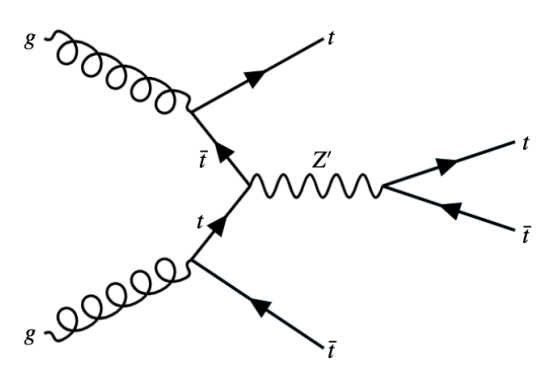
\includegraphics[width=0.32\linewidth]{fig/theory_ttZp.png}}
\subfloat[$tjZ'$]{
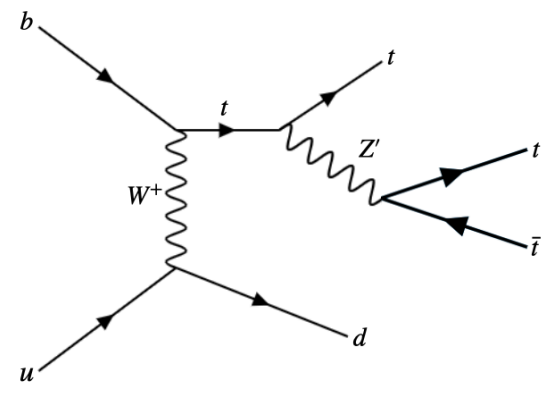
\includegraphics[width=0.32\linewidth]{fig/theory_tjZp.png}}
\subfloat[$tWZ'$]{
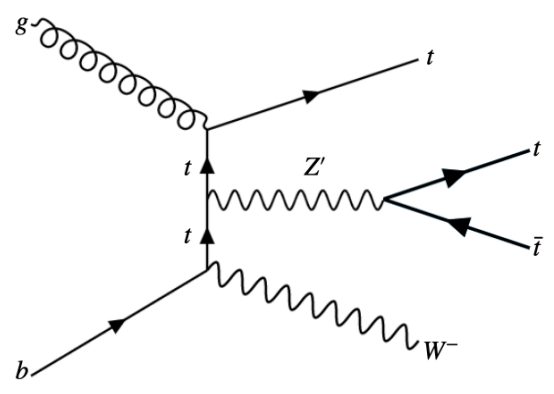
\includegraphics[width=0.32\linewidth]{fig/theory_tWZp.png}}
\caption[Feynman diagrams for tree level $Z'$ production in association with (a) \ttbar, (b) $tj$ (light quark) and (c) $tW$, decaying to final states containing (a) \tttt or (b)(c) \ttt.]{\label{fig:theory:ttZp_feynman}Feynman diagrams for tree level $Z'$ production in association with (a) \ttbar, (b) $tj$ (light quark) and (c) $tW$, decaying to final states containing (a) \tttt or (b)(c) \ttt \citep{theory:ttZp}.}
\end{figure}

The single-top-associated channels $tjZ'$ and $tWZ'$ are suppressed by three-body phase space \citep{theory:ttZp}, resulting in smaller cross sections by a factor of two compared to the \ttbar-associated process \ttZp. Unlike $tjZ'$ and $tWZ'$ which are produced via \acs{EW} and mixed \acs{QCD}-\acs{EW} interactions respectively, \tttt production is governed by the strong interaction which can overpower phase space suppression. Additionally, \tttt production is independent of $\theta$ while $tjZ'$ and $tWZ'$ are minimally suppressed under pure left-handed interactions ($\theta=0$) and maximally suppressed under pure right-handed interactions ($\theta=\pi/2$).

\subsection{\acs{BSM} four-top quark production}
\label{sec:4top}
This analysis uses the \tttt final state signal signature to search for the existence of a heavy \acs{BSM} resonance that couples strongly to the top quark. Cross section for \tttt production can be enhanced by many possible \acs{BSM} models, in particular two-Higgs-doublet-models \citep{Branco:2011iw,PhysRevD.93.075038,higgscomp} (2HDM) or possible production of a heavy neutral resonance boson $Z'$($\rightarrow\ttbar$) in association with a \ttbar pair in composite Higgs scenarios \citep{Ferretti:2013kya,Vecchi:2015fma}. The \ttZp production mode and consequently \tttt signal signature can provide a more sensitive channel for searches by avoiding contamination from the large \acs{SM} $gg\rightarrow \ttbar$ background in an inclusive $Z'\rightarrow\ttbar$ search.

\subsection*{Decay modes}
The different $W$ boson decay modes shown in \autoref{fig:theory:tt_decay} result in many different final states for \ttZp/\tttt decay, which can each be classified into one of three channels: all hadronic decays; exactly one lepton or two opposite-sign leptons (\acs{1LOS}); exactly two same-sign leptons or three or more leptons (\acs{SSML}). The branching ratio for each channel is shown in \autoref{fig:theory:tttt_channels}. The all hadronic and \acs{1LOS} channels have much larger branching ratios compared to \acs{SSML} channel but suffer heavily from $gg\rightarrow\ttbar$ background contamination, giving the \acs{SSML} channel better sensitivity at the cost of lower statistics. This is also the targeted channel for this analysis.

%\begin{wrapfigure}{r}{0.48\textwidth}
\begin{figure}[!htb]
\begin{center}
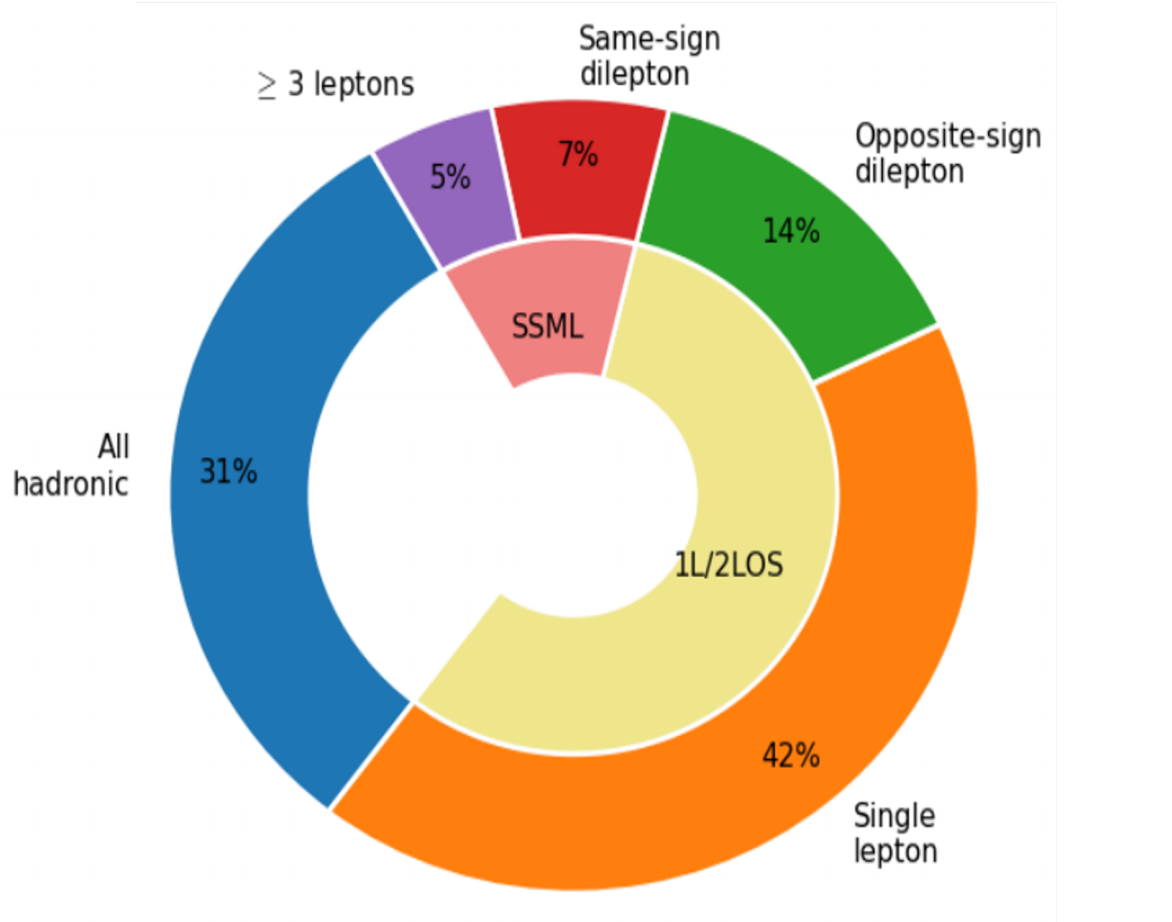
\includegraphics[width=0.7\linewidth]{fig/theory_tttt_channels.png}
\caption[Branching ratios for \tttt decay. The same-sign dilepton and multilepton channels together forms the SSML channel.]{\label{fig:theory:tttt_channels}Branching ratios for \tttt decay \citep{Sabatini:2784150}. The same-sign dilepton and multilepton channels together forms the \acs{SSML} channel.}
\end{center}
\end{figure}
%\end{wrapfigure}

%\begin{figure}[!htb]
%\begin{center}
%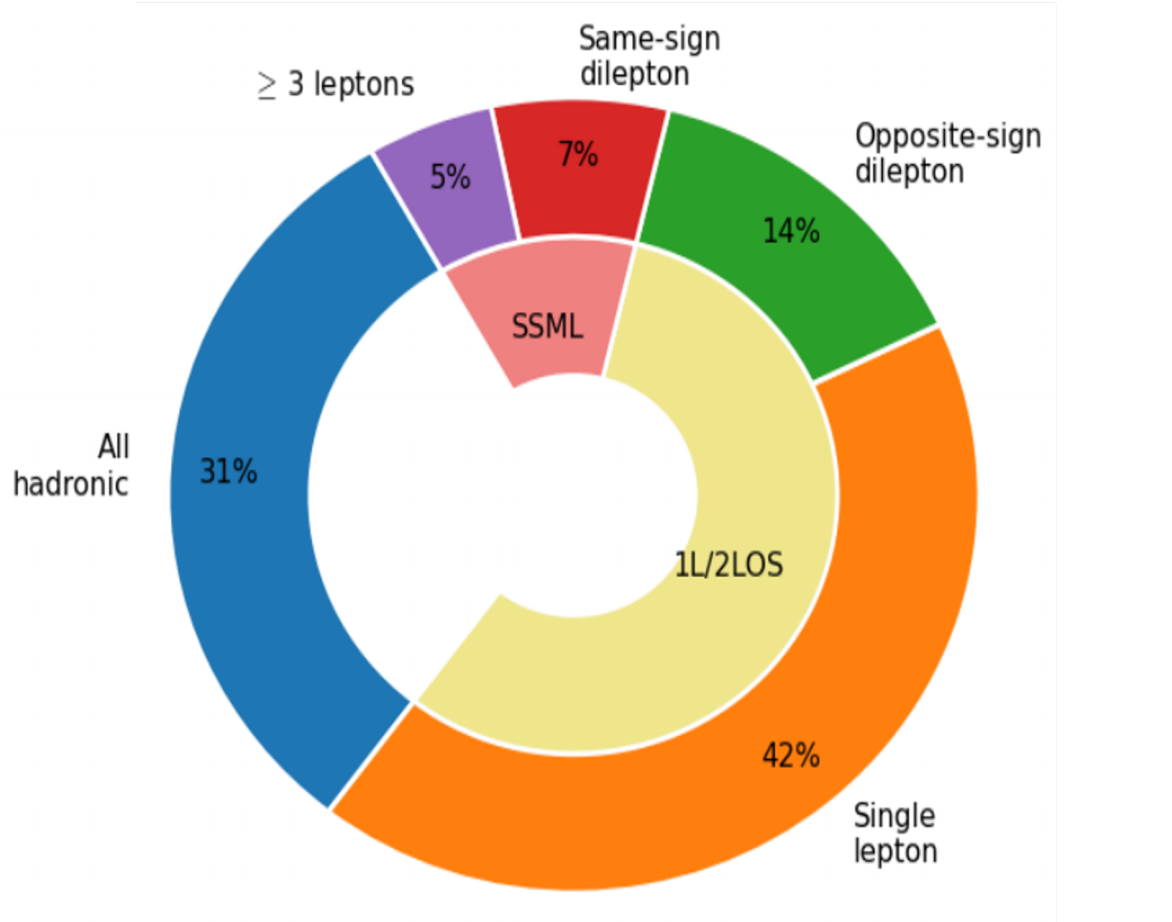
\includegraphics[width=0.6\linewidth]{fig/theory_tttt_channels.png}
%\caption{\label{fig:theory:tttt_channels}Caption}
%\end{center}
%\end{figure}

%\subsection*{Higgs-top Yukawa coupling}
%(show Lagrangian of Higgs-top Yukawa coupling)\\
%(show dependence of \tttt xsec on Yukawa coupling at LO)


%\section{Collider physics}
%[pp collision, pdf, cross section, luminosity]
%\subsection*{Luminosity}
%\subsection*{Proton-proton collisions}
%jets, parton shower, hadronization
%\subsection*{Parton distribution function}
%\subsection*{Cross section}


\end{document}